%%!TEX TS-program = latex

\documentclass[aps,pra,onecolumn]{revtex4-2}
\usepackage{amsmath,amsfonts,amsthm,bbm}
\usepackage[dvipsnames]{xcolor}
\usepackage{graphicx}
\usepackage{multirow,mhchem,chemformula}
\usepackage[colorlinks=true,breaklinks=true,linkcolor=red,citecolor=magenta,urlcolor=magenta]{hyperref}

\usepackage{tikz}
\usetikzlibrary{quantikz}

\newcommand{\crt}[1]{\hat{c}_{#1}^\dagger}
\newcommand{\dst}[1]{\hat{c}_{#1}^{\phantom{\dagger}}}
\newcommand{\vett}[1]{{\bf{#1}}}
\newcommand{\bgreek}[1]{{\boldsymbol{#1}}}
\newcommand{\ry}{R_y}
\newcommand{\ang}{\mathrm{\AA}}
\newcommand{\todo}[1]{{\bf{{\color{red}TODO: #1}}}}


\begin{document}

\title{Accuracy assessment of variational quantum computing Ans\"{a}tze \\
across a database of electronic structure problems}

\author{IBM authors}
\affiliation{IBM Quantum, IBM Research Almaden, 650 Harry Road, San Jose, CA 95120, USA}
\author{Virginia Tech authors}
\affiliation{Department of Chemistry, Virginia Tech, 480 Davidson Hall, Blacksburg, VA 24061, USA}

\begin{abstract}
\todo{abstract}
\end{abstract}

\maketitle

\section{Introduction}

Recent years have witnessed remarkable research in the simulation of many-body quantum systems  by quantum computing algorithms.
A prominent application targeted by quantum algorithms is the electronic structure (ES) problem, 
namely solving for the ground or low-lying eigenstates of the electronic Schr\"{o}dinger equation for atoms, molecules, and materials.
Research in this direction has delivered promising results in the calculation of potential energy curves,
ground- and excited-state energies, and correlation functions for various instances of the ES problem.

Notwithstanding these rapid developments, the behavior of quantum computing algorithms for the ES problem remains to be understood and established,
and such a situation is due to several factors. For example: 
different research groups demonstrate existing or novel algorithms on different instances of the ES problem, which makes comparative algorithm analysis difficult;
the design and implementation of novel quantum computing algorithms is often coupled to their demonstration on contemporary quantum hardware, which restricts the domain of potential applications to very small numbers of electrons and orbitals;
the limitations of classical simulators have similarly resulted in most simulations reported to date being restricted to very small instances of the ES problem, so that the observed algorithmic behavior is not guaranteed to generalize to larger or more complex instances;
even when quantum algorithms have known limitations, their numeric assessment is often limited by the immaturity of contemporary quantum computational platforms, which makes difficult to gauge the severity of such limitations.

Overcoming these limiting factors can contribute to the understanding of the nature, performance and limitations of quantum algorithms for the ES problem, and bring progress in their design and assessment.
Useful steps towards this goal are:
to establish a database of problems that different researchers can use to test quantum algorithms;
to propose a set of metrics to quantify algorithmic performance, and support an objective comparison of algorithmic behavior;
to establish a database of results that different researchers can consult to compare and contrast quantum algorithms.

The proposed problems should be sufficiently simple, to be demonstrated on contemporary quantum computing platforms, and non-trivial, to ensure meaningful assessments of algorithmic behavior.
Moreover, the assessment of algorithmic behavior should decouple classical simulators of quantum devices and actual quantum devices,
so that theoreticians can explore the properties of a methodology assuming an ideal quantum device, and experimentalists can independently test a set of well-defined quantum circuits motivated by the solution of instances of the ES problem.
 
In this work, we present a set of instances of the ES problem, and perform an assessment of Ans\"{a}tze used in variational ground-state quantum simulations,
using classical simulators of quantum hardware.
In the assessment of quantum algorithms, we will use the difference between the computed and exact ground-state energy as an indicator of algorithmic quality,
along with the expectation values of quantities signaling the breaking of Hamiltonian symmetries, a conceptually important but often overlooked aspect of variational quantum simulations.
We will use a variety of indicators of algorithmic cost, related to the optimization of variational parameters (number of variational parameters, cost of energy evaluation)
and to the quantum circuits leading to the calculation of energies and properties (number of qubits, gates, circuit depth).

As illustrative applications, we employ the database presented here to test a new variational Ansatz termed {\em{cascade}} against existing methods,
to compare open- and closed-shell implementations of the unitary coupled-cluster with singles and doubles \cite{scuseria1987closed,szalay1997spin}, 
and to compare two different strategies to encode fermionic degrees of freedom to qubits.

The remainder of this work is organized as follows: 
in Section \ref{sec:methods} we describe the proposed database, and the algorithms tested in the present work;
in Section \ref{sec:results} we present the results of this study;
conclusions and perspective prosecutions of this work are describe in Section \ref{sec:conclusions},
and an appendix contains additional computational details.

\section{Methods}
\label{sec:methods}

In this section, we present the problems constituting the database studied in this work,
and the metrics used to establish algorithm performance and computational cost.

\subsection{Target problems}

In this work, we focus on a set of four molecular species, namely BH, HF, BeH$_2$, and H$_2$O.
The BH, HF, BeH and OH bondlengths $R$ vary between 0.7 and 3.5, 4.5, 4.5, and 3.3 $\ang$ respectively.
These molecular species, proposed in previous works, allow to test quantum algorithms along the breaking of one (BH and HF) or two (BeH$_2$, and H$_2$O) covalent bonds,
and in presence of dominant dynamic (small $R$) or static (large $R$) electronic correlation.

For each species, a restricted closed-shell Hartree-Fock calculation is performed, as specified in Appendix \ref{sec:classical}.
The core 1s orbital is frozen and the Born-Oppenheimer Hamiltonian
\begin{equation}
\label{eq:hamiltonian}
\hat{H} = E_0 + \sum_{\substack{p r \\ \sigma}} h_{p r} \crt{p \sigma} \dst{r \sigma} + \sum_{\substack{p r q s \\ \sigma\tau}} \frac{(pr|qs)}{2} \crt{p \sigma} \crt{q \tau} \dst{s\tau}  \dst{r \sigma}
\end{equation}
is computed, along with the number, spin-$z$, and total spin operators
\begin{equation}
\label{eq:auxiliary}
\begin{split}
\hat{N} &= N_f + \sum_{p \sigma} \crt{p \sigma} \dst{p \sigma} \quad, \\
\hat{S}_z &= \sum_{p \sigma} (-1)^\sigma \crt{p \sigma} \dst{p \sigma} \quad, \\
\hat{S}^2 &= \sum_{pq} \crt{p\downarrow} \dst{p\uparrow} \crt{q\uparrow} \dst{q\downarrow}   + \hat{S}_z (\hat{S}_z-1) \quad,
\end{split}
\end{equation}
where $N_f = 2$ is the number of frozen electrons. 
In this study we focused on a minimal STO-6G basis, to ensure a number of orbitals and qubits within the reach of contemporary classical simulators of quantum circuits.

\subsection{Qubit encodings}

In the majority of quantum algorithms for contemporary devices, the Hamiltonian Eq.~\eqref{eq:hamiltonian} and the auxiliary operators Eq.~\eqref{eq:auxiliary} are mapped onto qubit operators,
and more specifically onto linear combinations 
\begin{equation}
\label{eq:qubit}
\hat{H} = \sum_{i=0}^{n_p-1} c_i \, \sigma_{\vett{v}_i \, \vett{w}_i} 
\quad,\quad
\sigma_{\vett{v} \, \vett{w}} = \bigotimes_{k=0}^{n_q-1} \sigma_{v_k w_k} 
\quad,
\end{equation}
of Pauli operators acting on a certain number $n_q$ of qubits. In Equation~\eqref{eq:qubit} $\sigma_{00,01,10,11} = \mathbbm{1},X,Z,Y$ is a single-qubit Pauli operator, 
$c_i$ a real-valued coefficient, and the summation ranges over $n_p$ terms.

In this study, we employ both second-quantization and first-quantization encodings.
The former establish a one-to-one mapping between the Fock space of electrons in $M$ spatial orbitals and the Hilbert space of $n_q = 2M$ qubits,
and the latter between the Hilbert space spanned by a set of $K$ space- and spin-adapted configuration state functions (CSFs) and the Hilbert space of $n_q = \lceil \log_2 K \rceil$ qubits.

First-quantization encodings ensure access to automatically symmetry-adapted many-electron wavefunctions, and require less qubits than their second-quantization counterparts.
However, they are less straightforward to implement, and lead to a representation of the Hamiltonian where $n_p$ scales exponentially with $n_q$.
Additional technical details are provided in Appendix \ref{sec:first}.

Second-quantization encodings give rise to a compact representation of the Hamiltonian and of auxiliary operators as linear combinations of a polynomial number of Pauli operators,
but allow the possibility that Hamiltonian symmetries are broken, for multiple reasons discussed in Section \ref{sec:metrics}.
To alleviate the latter issue, we combine the parity mapping with the two-qubit and tapering techniques. The former removes two qubits to ensure conservation of the parity operators
$(-1)^{\hat{N}_\uparrow}$ and $(-1)^{\hat{N}_\downarrow}$, and the latter identifies a subgroup of the symmetry group isomorphic to $\mathbb{Z}_2^{\times k}$ and removes $k$ qubits
to ensure the simulated wavefunctions lie in a target irrep of the identified subgroup. The species studied here have symmetry groups 
($C_{\infty v}$ for BH and HF, $D_{\infty h}$ for BeH$_2$ and $C_{2v}$ for H$_2$O) isomorphic to $\mathbb{Z}_2 \times \mathbb{Z}_2$, so that the combined use of two-qubit reduction
and tapering leads to $n_q = 2M-4$ qubits.

\subsection{Target variational Ans\"{a}tze}

In this study, we elected to explore the behavior of the variational quantum eigensolver (VQE) algorithm, due to its widespread adoption in the community.
This method defines a set of Ansatz states approximating the ground state of a target Hamiltonian, of the form 
\begin{equation}
| \Psi( \bgreek{\theta} ) \rangle = \hat{U}( \bgreek{\theta} ) | 0 \rangle^{\otimes n_q}
\quad,
\end{equation}
where $\bgreek{\theta} \in [0,2\pi)^{n_\theta}$ is an array of angles that define a parametrized quantum circuit $\hat{U}( \bgreek{\theta} )$, 
applied to a register of $n_q$ qubits prepared in the standard initial state $| 0 \rangle^{\otimes n_q}$.
The best approximation to the ground state in the set of Ansatz states is found by minimizing the energy 
\begin{equation}
E_{\mathrm{VQE}}( \bgreek{\theta} ) = \langle \Psi( \bgreek{\theta} ) | \hat{H} | \Psi( \bgreek{\theta} ) \rangle
\end{equation}
as a function of the parameters $\bgreek{\theta} $ using a classical optimization algorithm. 
Once the parameters are optimized, auxiliary observables can be measured, yielding results
\begin{equation}
X_{\mathrm{VQE}}( \bgreek{\theta} ) = \langle \Psi( \bgreek{\theta} ) | \hat{X} | \Psi( \bgreek{\theta} ) \rangle
\quad.
\end{equation}
This algorithmic workflow, termed variational quantum eigensolver (VQE) in the quantum simulation literature, 
is a heuristic technique for ground-state approximation. 
Its accuracy and computational cost, as discussed in Section \ref{sec:metrics}, are determined by the details of the circuit $\hat{U}( \bgreek{\theta} )$. 
In the remainder of this Section, we will present the Ans\"{a}tze assessed in the present work.

\subsubsection{Unitary coupled cluster with singles and doubles}

The quantum unitary coupled cluster (q-UCC) method is based on the exponential Ansatz, i.e., the exact wave function is written as
\begin{equation}
| \Psi_{\mathrm{gs}} \rangle = e^{ \hat{T} - \hat{T}^\dagger } | \Phi_0 \rangle
\end{equation}
where $\Phi_0$ is an independent particle function (here, the Hartree-Fock state) and $\hat{T}$ is a cluster operator which, 
at the singles and doubles level (q-UCCSD) is truncated to
\begin{equation}
\label{eq:unrestricted_quccsd}
\begin{split}
\hat{T} &= \hat{T}_1 + \hat{T}_2 \quad, \\
\hat{T}_1 &= \sum_{\substack{ai \\ \sigma}} t^{a \sigma}_{i \sigma} \crt{a \sigma} \dst{i \sigma} \quad,\\
\hat{T}_2 &= \sum_{\substack{abij \\ \sigma\tau}} t^{a\sigma \; b\tau}_{i\sigma \; j\tau} \crt{a \sigma} \crt{b \tau} \dst{j \tau} \dst{i \sigma} \quad,\\
\end{split}
\end{equation}
where $t^{a}_i$ and $t^{ab}_{ij}$ are a set of unknown cluster coefficients. We have adopted the convention that $i,j,k,l$ and $a,b,c,d$
refer to occupied and unoccupied orbitals in the reference configuration $\Phi_0$ respectively.
It should be noted that the form Eq.~\eqref{eq:unrestricted_quccsd}, presented in previous literature along with the corresponding quantum circuit,
corresponds to an unrestricted Ansatz, which is not guaranteed to yield an eigenfunction of total spin.

If a closed shell spin-adapted formalism is used, then, following Paldus and Scuseria et al, we need to have
\begin{equation}
t^{a \alpha}_{i \alpha} = t^{a \beta}_{i \beta} = t^a_i \quad,
\end{equation}
since the two other possible spin combinations are vanishing. 
Only 6 of the 16 possible spin combinations for the two-electron amplitudes are non-zero, namely
\begin{equation}
\begin{split}
t^{a \alpha \; b \alpha}_{i \alpha \; j \alpha} = t^{a \beta \; b \beta}_{i \beta\; j\beta} = \hat{t}^{ab}_{ij} \\
t^{a \alpha \; b \beta}_{i \alpha \; j \beta} = t^{a \beta \; b \alpha}_{i \beta\; j\alpha} = \tilde{t}^{ab}_{ij} \\
t^{a \beta \; b \alpha}_{i \alpha \; j \beta} = t^{a \alpha \; b \beta}_{i \beta\; j\alpha} = \overline{t}^{ab}_{ij} \\
\end{split}
\end{equation}
Using the relations
\begin{equation}
\hat{t}^{ab}_{ij} = \tilde{t}^{ab}_{ij} + \overline{t}^{ab}_{ij}
\quad,\quad
\tilde{t}^{ab}_{ij} = - \overline{t}^{ab}_{ji} = - \overline{t}^{ab}_{ij} = \tilde{t}^{ba}_{ji}
\quad,
\end{equation}
one is left with only one set of independent two-electron amplitudes $\tilde{t}^{ab}_{ij}$ and $(ai) \leq (bj)$. In addition to reducing the 
number of variational parameters, the use of a closed shell spin-adapted formalism ensures that the cluster operator commutes with 
the total spin operator, $[ \hat{T} , \hat{S}^2 ] = 0$.
Its exponential, however, cannot be implemented exactly at polynomial cost on a quantum computer. 
Instead, as discussed in Appendix \ref{sec:cc_trotter}, a Trotter approximation is required, which in turn leads to spin symmetry breaking.
Appendix \ref{sec:cc_trotter} also shows the quantum circuits used to implement the q-UCCSD Ansatz in a Jordan-Wigner representation.

% fare

\subsubsection{Hardware-efficient $\ry$}

Hardware-efficient Ans\"{a}tze are families of wavefunctions designed with the primary goal to be compatible with the budget of contemporary quantum hardware 
in terms of available qubits, connectivity, native gates, and circuit depth.
An example is the following $\ry$ Ansatz,
\begin{equation}
| \Psi(\theta) \rangle = 
\prod_{k=1}^{n_r}
\left(
\prod_{i=0}^{n_q-1} R_{y,i}(\theta_{k,i})
\prod_{ij\in C} G_{ij}
\right)
\prod_{i=0}^{n_q-1} R_{y,i}(\theta_{0,i}) | \Psi_0 \rangle
\;,
\end{equation}
where $| \Psi_0 \rangle$ is an initial wavefunction (here, the restricted 
closed-shell Hartree-Fock state), $n_q$ is the number of qubits, $R_{y,i}(\theta) 
= \mbox{exp}(-i \theta Y_i/2)$ is a $Y$ rotation of an angle $\theta$ 
applied to qubit $i$, $G_{ij}$ a parameter-free two-qubit entangling 
gate (here, the CNOT gate) applied to a pair $(ij)$ of connected qubits,
and $n_r$ is an integer denoting the number of times a layer of entangling gates
followed by a layer of $Y$ rotations is repeated.
Here, we focused on the {\em{linear-connectivity}} and {\em{full-connectivity}} $\ry$ Ans\"{a}tze, respectively given by
\begin{equation}
\label{eq:ry_connectivity}
C_{\mathrm{linear}} = \{ (i,i+1) \;,\; i = 0 \dots n_q-2 \}
\quad,\quad
C_{\mathrm{full}} = \{ (i,j) \;,\; i = 0 \dots n_q-1 \;,\; j \geq i \}
\quad.
\end{equation}
Examples of linear- and full-connectivity $\ry$ Ans\"{a}tze are shown in Figure \ref{figure:ry}. 
It is worth observing that other choices of connectivity are possible, and that Eq.~\eqref{eq:ry_connectivity} exemplifies
two opposite regimes.

\begin{figure}[t!]
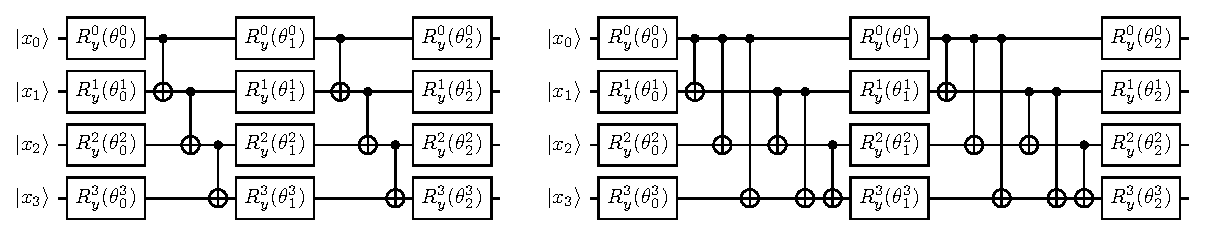
\includegraphics[width=0.85\textwidth]{../figures/circuits/ry.eps}
\caption{Quantum circuits implementing the linear- and full-connectivity $\ry$ Ansatz, with $n_q=4$ qubits and $n_r=2$ repetitions (left, right respectively).}
\label{figure:ry}
\end{figure} 

\subsubsection{Cascade}

In standard qubit representations, the Hartree-Fock state is mapped onto a computational basis state, or a bit-string, $| \Psi_0 \rangle = \otimes_{i=0}^{n_q-1} |x_i \rangle = | {\bf{x}} \rangle$.
When applied to an initial state of the form $| \Psi_0 \rangle = | {\bf{x}} \rangle$, the $\ry$ Ansatz with $\bgreek{\theta} = {\bf{0}}$ returns a bitstring $| {\bf{x}}^\prime \rangle$ potentially with
different properties than $| {\bf{x}} \rangle$, e.g. higher energy, higher/lower particle number. 

In some situations, it is desirable to employ Ans\"{a}tze with the property that $\hat{U}({\bf{0}}) = \mathbbm{1}$, so that the starting point of the optimization is the Hartree-Fock state.
An example is the following Ansatz, that we term "cascade",
\begin{equation}
| \Psi(\bgreek{\theta}) \rangle 
= \prod_{k=1}^{n_r}
\left(
\prod_{i=0}^{n_q-1} R_{y,i}(\theta_{k,n_q+i})
\;
C^\dagger
\;
\prod_{i=0}^{n_q-1} R_{y,i}(\theta_{k,i})
\;
C
\right)
\prod_{i=0}^{n_q-1} R_{y,i}(\theta_{0,i}) | \Psi_0 \rangle
\quad,\quad
C = \prod_{i=0}^{n_q-2} \mathsf{c}_i X_{i+1}
\quad.
\end{equation}
The cascade Ansatz is illustrated in Figure \ref{figure:cascade}. As seen, the presence of $C$ and $C^\dagger$ ensures that $\hat{U}({\bf{0}}) = \mathbbm{1}$.
Furthermore, as in other Ans\"{a}tze \cite{qaoa,qubit_cc}, given a wavefunction with $n_r$ repetitions and optimized parameters $\bgreek{\theta}_{n_r}$, 
a wavefunction with $n_r+1$ repetitions can be initialized from the parameter configuration $\bgreek{\theta}_{n_r+1} = ( \bgreek{\theta}_{n_r} , {\bf{0}} )$ 
so that the VQE energy decreases monotonically with $n_r$.
 
\begin{figure}[t!]
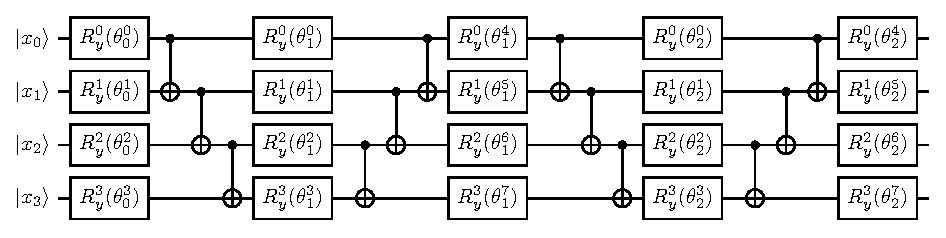
\includegraphics[width=0.7\textwidth]{../figures/circuits/cascade.eps}
\caption{Quantum circuit implementing the cascade Ansatz, with $n_q=4$ qubits and $n_r=2$ repetitions.}
\label{figure:cascade}
\end{figure} 

\subsection{Metrics of algorithm performance}
\label{sec:metrics}

A natural metric to assess the accuracy of a variational simulation is the difference between the computed and exact ground-state energy, 
\begin{equation}
\Delta E = E_{\mathrm{VQE}}(\bgreek{\theta}) - E_{\mathrm{FCI}}
\quad .
\end{equation}
The ES Hamiltonian has several symmetries, i.e. operators $\hat{S}$ such that $[\hat{H},\hat{S}]=0$. 
In presence of Hamiltonian symmetries, the search for Hamiltonian eigenfunctions has to be restricted to eigenspaces of Hamiltonian symmetries with known eigenvalues.
Relevant Hamiltonian symmetries are the auxiliary operators Eq.~\eqref{eq:auxiliary}
and, for the molecules studied in the present work, the ground state lies in the eigenspaces of $\hat{S}_z$ and $\hat{S}^2$ with eigenvalue zero,
and of $\hat{N}$ with eigenvalues $6$ for BH and BeH$_2$ and 10 for HF and H$_2$O.

In general, a variational quantum simulation does not preserve Hamiltonian symmetries. To assess whether a variational simulation
leads to symmetry breaking, and to quantify its extent, we compute the deviations
\begin{equation}
\begin{split}
\Delta N &= N_{\mathrm{VQE}}(\bgreek{\theta}) - N_{\mathrm{FCI}} \quad, \\
\Delta S_z &= S_{z,\mathrm{VQE}}(\bgreek{\theta}) - S_{z,\mathrm{FCI}} \quad, \\
\Delta S^2 &= S^2_{\mathrm{VQE}}(\bgreek{\theta}) - S^2_{\mathrm{FCI}} \quad, \\
\end{split}
\end{equation}
between the computed and exact ground-state particle number, spin-$z$, and total spin.

In addition to the accuracy of a variational simulation, it is also important to quantify its computational cost. To this end we employ a tuple of values,
namely: 
the number of qubits $n_q$,  
the number of repetitions $n_r$,  
the number of gates $n_g$ and the depth $d$ of the variational circuit, 
the number of Pauli operators in the Hamiltonian $n_p$, 
and the number of variational parameters $n_{\bgreek{\theta}}$.

\section{Results}
\label{sec:results}

The overall strategy for the calculations performed in this work involved initial pre-processing by classical quantum chemistry codes on conventional computers, 
to generate optimized Hartree-Fock orbitals and matrix elements of the Hamiltonian, prior to performing computations with quantum simulators or devices.
The restricted Hartree-Fock (RHF) singlet state has been chosen as the initial state for all of the calculations described here, 
since experience has indicated this state as a good choice for a variety of chemical problems \cite{romero2018strategies}. 
Details about the molecular orbitals are shown in Figure \ref{figure:scf} of the Appendix.

Having selected a set of single-electron orbitals for each of the studied species, VQE computations were performed with quantum simulators and devices. 
We use IBM's open-source Python library for quantum computing, Qiskit \cite{aleksandrowicz2019qiskit}. 
Qiskit provides tools for various tasks such as creating quantum circuits and performing simulations. 
In particular, it contains an implementation of the VQE algorithm, and a classical exact eigensolver algorithm to compare results.
Details about the natural orbitals from classical exact eigensolver calculations are shown in Figure \ref{figure:scf} of the Appendix.

We then minimize the expectation value of the Hamiltonian with respect to the parameters of our circuit. 
The minimization is carried out through the classical optimization method, L$\_$BFGS$\_$B \cite{zhu1997algorithm,byrd1995limited,morales2011remark}.

Once the VQE is complete, we obtain the optimized variational form and the estimate for the ground state energy. 
In addition, we measure a set of auxiliary operators.

The results illustrated in this study are stored in a publicly available Github repository, organized as detailed in Appendix \ref{sec:github}.

\subsection{Second-quantization simulations}

\begin{figure}[t!]
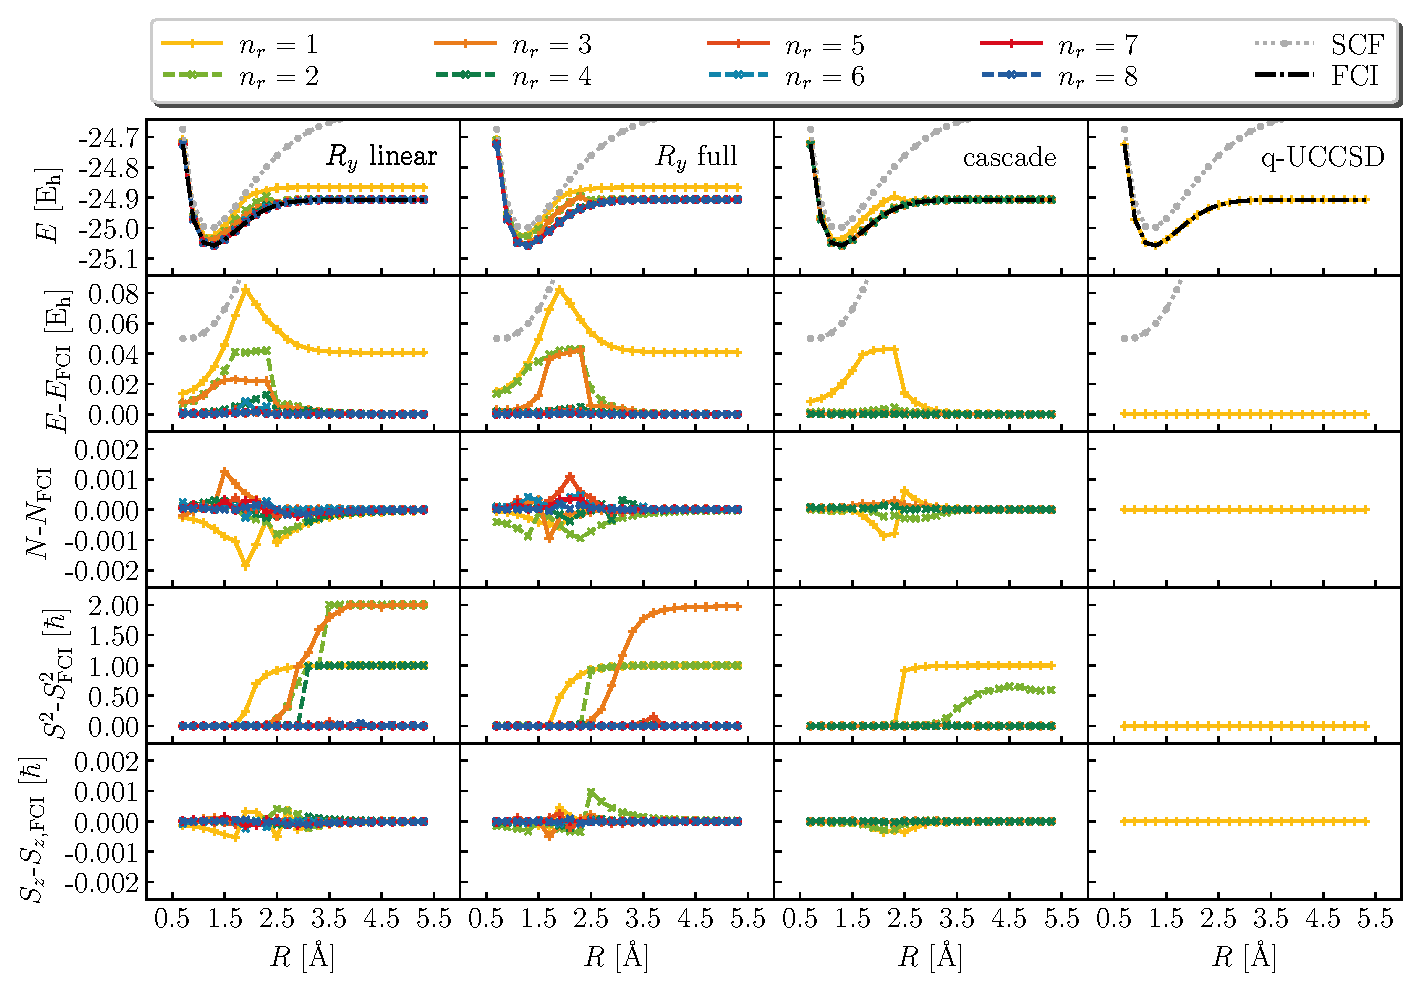
\includegraphics[width=0.8\textwidth]{../figures/second_quantization_bh/second_quantization_bh.eps}
\caption{Total energy, deviation between computed and exact total energy, electron number, total spin, and spin-$z$ (top to bottom) 
using the R$_y$ (with linear and full connectivity), cascade, and q-UCCSD Ans\"{a}tze (left to right), for the BH molecule at STO-6G level.
}
\label{figure:second_bh}
\end{figure}

\begin{figure}[t!]
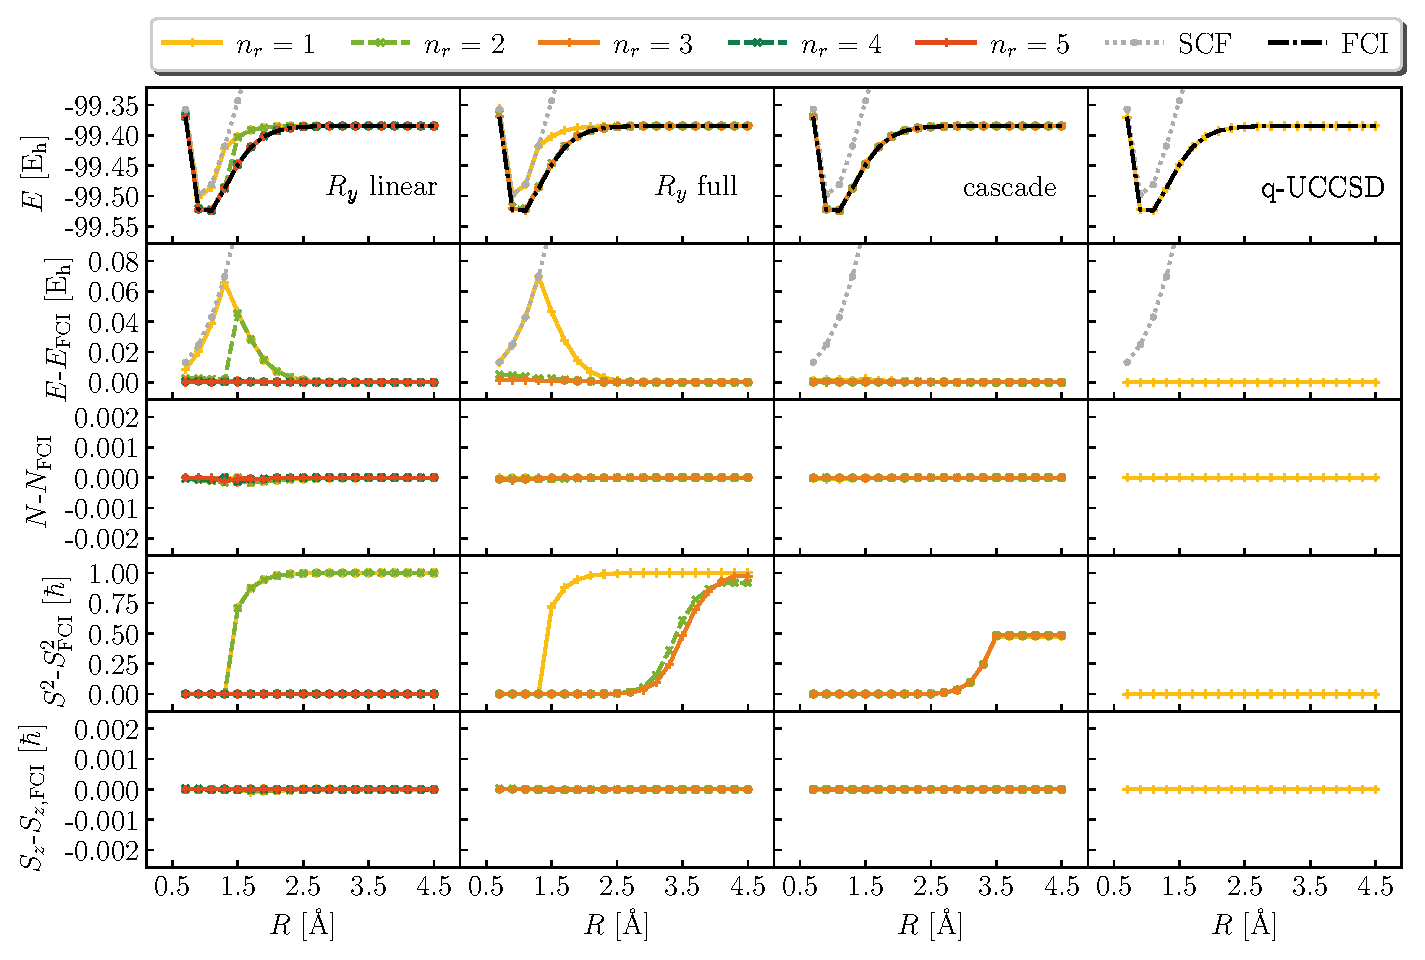
\includegraphics[width=0.8\textwidth]{../figures/second_quantization_hf/second_quantization_hf.eps}
\caption{Total energy, deviation between computed and exact total energy, electron number, total spin, and spin-$z$ (top to bottom) 
using the R$_y$ (with linear and full connectivity), cascade, and q-UCCSD Ans\"{a}tze (left to right), for the HF molecule at STO-6G level.}
\label{figure:second_hf}
\end{figure}

\begin{figure}[t!]
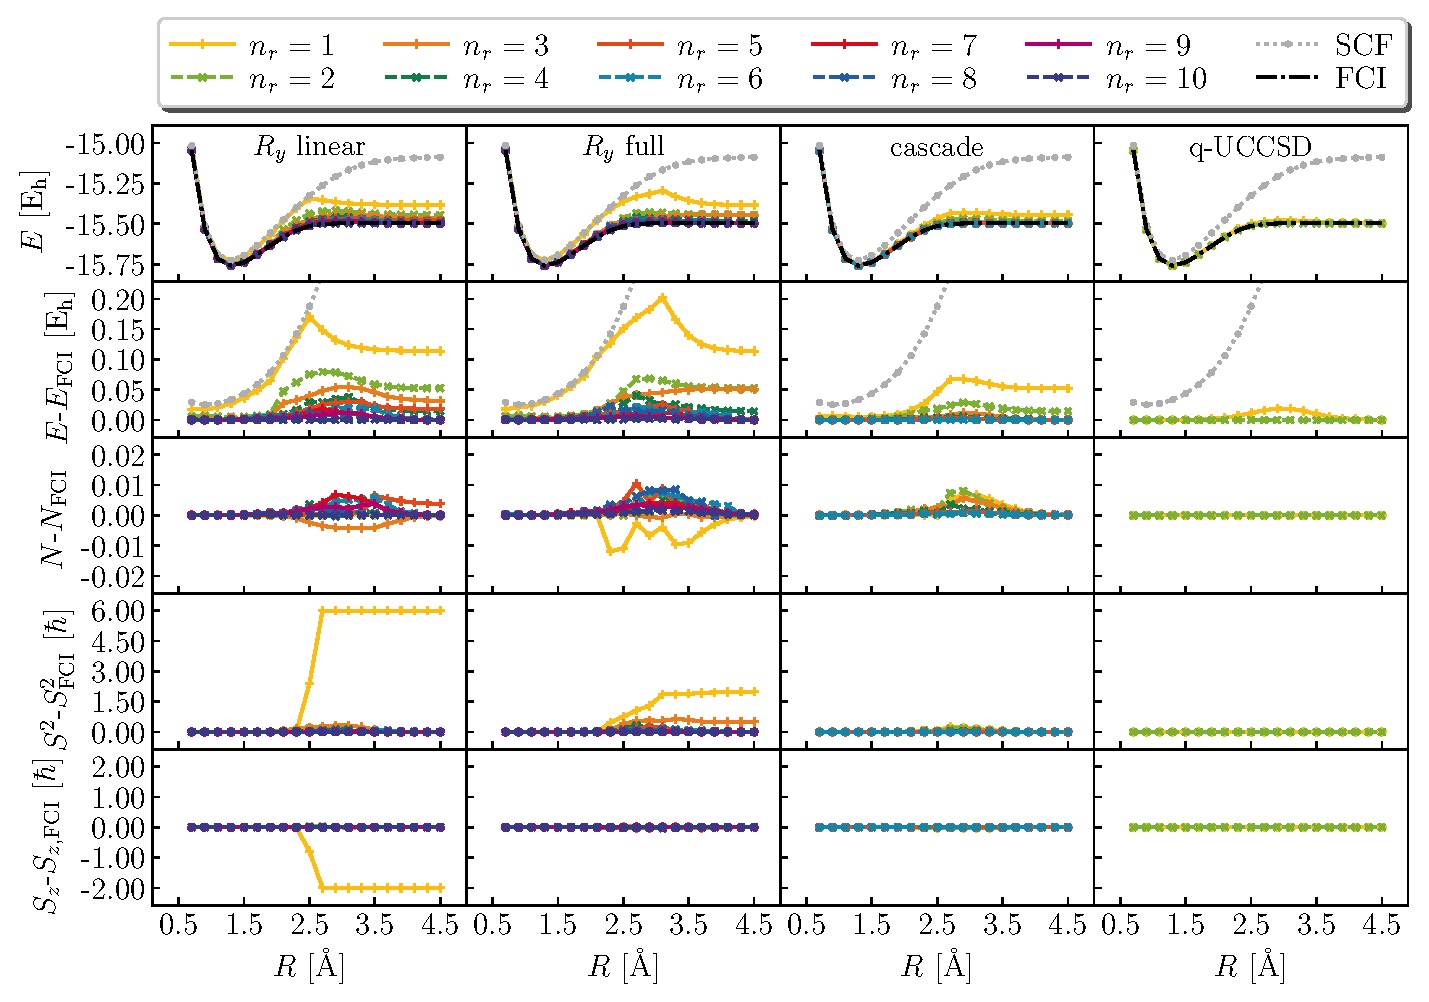
\includegraphics[width=0.8\textwidth]{../figures/second_quantization_beh2/second_quantization_beh2.eps}
\caption{Total energy, deviation between computed and exact total energy, electron number, total spin, and spin-$z$ (top to bottom) 
using the R$_y$ (with linear and full connectivity), cascade, and q-UCCSD Ans\"{a}tze (left to right), for the BeH$_2$ molecule at STO-6G level.
}
\label{figure:second_beh2}
\end{figure}

\begin{figure}[t!]
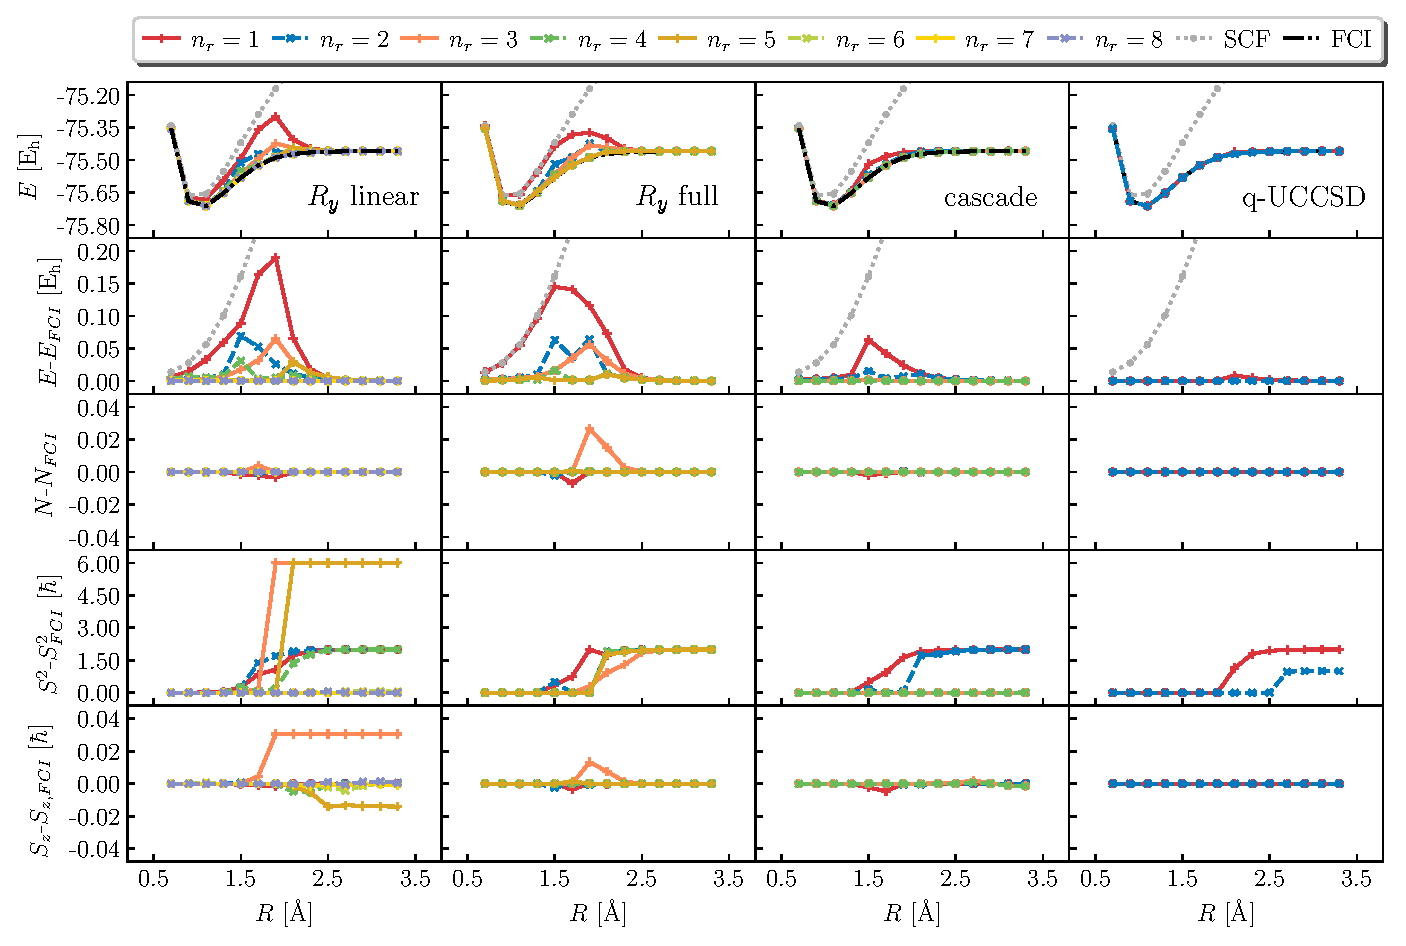
\includegraphics[width=0.8\textwidth]{../figures/second_quantization_h2o/second_quantization_h2o.eps}
\caption{Total energy, deviation between computed and exact total energy, electron number, total spin, and spin-$z$ (top to bottom) 
using the R$_y$ (with linear and full connectivity), cascade, and q-UCCSD Ans\"{a}tze (left to right), for the H$_2$O molecule at STO-6G level.}
\label{figure:second_h2o}
\end{figure} 


In Figures \ref{figure:second_bh}, \ref{figure:second_hf}, \ref{figure:second_beh2}, and \ref{figure:second_h2o} we compute ground-state potential energy curves
for the BH, HF, BeH$_2$, and H$_2$O molecules respectively, using a second-quantization encoding.

For all the studied molecules, bondlengths, and Ans\"{a}tze, energies typically decrease monotonically with Ansatz depth $n_r$. 
As naturally expected, the q-UCCSD Ansatz outperforms hardware-efficient Ans\"{a}tze, 
since it is constructed starting from the natural excitation of the system (i.e. electronic transition from occupied to virtual orbitals), rather than from application-agnostic circuits. 

The most challenging regime is the intermediate dissociation region ($R \simeq 2$-$3 \ang$), 
where the energies from hardware-efficient Ans\"{a}tze are more than 100 milliHartreee above the FCI value and clearly display cusps.
Such artifacts are especially pronounced for the H$_2$O and BeH$_2$ molecules, where two bonds are dissociated.

Interestingly, the linear-connectivity $\ry$ Ansatz typically outperforms its full-connectivity counterpart, achieving less inaccurate results with less quantum resources.
Furthermore, a cascade Ansatz with $n_r$ repetitions performs roughly as well as a linear-connectivity $\ry$ Ansatz with $2 n_r$ repetitions.

It should be noted that an inaccurate performance by hardware-efficient Ans\"{a}tze is accompanied by a pronounced breaking of the spin symmetry:
the total spin of low-depth $\ry$ Ans\"{a}tze evolves from $S^2 = 0$ at short $R$ towards either the triplet or quintuplet value ($S^2 = 2,6 \hbar$ respectively).
Ansatz inaccuracy and symmetry breaking, however, are not perfectly correlated: the largest deviations between VQE and FCI energies occur in the intermediate dissociation region,
where symmetry breaking start to develop; on the other hand, symmetry breaking is most pronounced at dissociation ($R \geq 3 \ang$),
where the VQE energy is in better agreement with FCI.

The computational costs of the second-quantization simulations shown in Figures \ref{figure:second_bh}, \ref{figure:second_hf}, \ref{figure:second_beh2}, \ref{figure:second_h2o} 
are listed in Table  \ref{table:computational_cost}.
 
\subsubsection{Comparison of calculations with highest $n_r$.}

Agreement with FCI within 1.6 milliHartree and smoother potential energy curves are only achieved by increasing $n_r$ to the values listed in Table \ref{table:nr_comparison}.
The energies of such Ans\"{a}tze are shown in Figure \ref{figure:second_comparison}.
The linear $\ry$, full-$\ry$ and cascade Ans\"{a}tze have $n_{\bgreek{\theta}} = n_q (n_r+1)$, $n_q (n_r+1)$, $n_q (2n_r+1)$ parameters respectively,
$n_g=(n_{\bgreek{\theta}},n_r n_q)$, $(n_{\bgreek{\theta}},n_r (n_q-1) n_q/2)$, $(n_{\bgreek{\theta}},2 n_r n_q)$ single-qubit and CNOT gates respectively,
and $d = n_r (n_q+1) +1$, $n_r (n_q-1) n_q/2 +1$, $n_r (2n_q+1) +1$ respectively. \todo{check once again}

\begin{table}[t!]
\begin{tabular}{ccccc|cccc}
\hline\hline
molecule & $n_e=(N_\alpha,N_\beta)$ & $m$ & $n_q$ & $n_p$ & ansatz & $n_{\bgreek{\theta}}$ & $n_g$ & $d$ \\ 
\hline
BH & (4,4) & 5 & 6 & 231 & $\ry$, linear & $12$ & $(14,5)$ & $8$ \\ 
  &   &  &   &   & $\ry$, full & $12$ & $(14,15)$ & $12$ \\ 
  &   &  &   &   & cascade & $18$ & $(20,10)$ & $14$ \\ 
  &   &  &   &   & q-UCCSD & $16$ & $(594, 552)$ & $740$ \\ 
\hline
HF & (4,4) & 5 & 6 & 231 & $\ry$, linear & $12$ & $(15, 5)$ & $8$ \\ 
  &   &  &   &   & $\ry$, full & $12$ & $(15, 15)$ & $12$ \\ 
  &   &  &   &   & cascade & $18$ & $(21,10)$ & $14$ \\ 
  &   &  &   &   & q-UCCSD & $10$ & $(451, 352)$ & $489$ \\ 
\hline
BeH$_2$ & (2,2) & 6 & 7 & 268 & $\ry$, linear & $14$ & $(15, 6)$ & $8$ \\ 
  &   &  &   &   & $\ry$, full & $14$ & $(15, 21)$ & $13$ \\ 
  &   &  &   &   & cascade & $21$ & $(22,12)$ & $15$ \\ 
  &   &  &   &   & q-UCCSD & $18$ & $(869, 808)$ & $1083$ \\ 
\hline
H$_2$O & (3,3) & 5 & 6 & 216 & $\ry$, linear & $12$ & $(15, 5)$ & $8$ \\ 
  &   &  &   &   & $\ry$, full & $12$ & $(15, 15)$ & $12$ \\ 
  &   &  &   &   & cascade & $18$ & $(21,10)$ & $14$ \\ 
  &   &  &   &   & q-UCCSD & $16$ & $(727, 636)$ & $896$ \\ 
\hline\hline
\end{tabular}
\caption{Computational cost of second-quantization simulations carried out in the present work. 
$n_e$, $m$, $n_q$, and $n_p$ denote numbers of active electrons (spin-up and -down) and orbitals, qubits, and Pauli operators in the Hamiltonian, respectively.
$n_{\bgreek{\theta}}$, $n_g$, and $d$ denote numbers of parameters, gates (single- and two-qubit), and circuit depth. For simplicity, we illustrate the case of $n_r=1$ repetitions.}
\label{table:computational_cost}
\end{table}

\begin{figure}[t!]
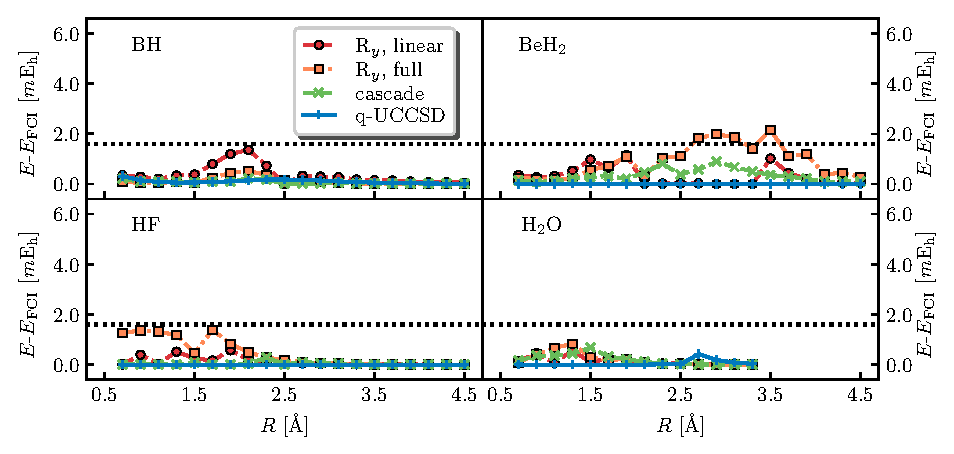
\includegraphics[width=0.7\textwidth]{../figures/second_quantization_comparison/second_quantization_comparison.eps}
\caption{Deviation between computed and exact total energy for the BH, HF, BeH$_2$ and H$_2$O molecules at STO-6G level 
(counterclockwise) using the R$_y$ (with linear and full connectivity), cascade, and q-UCCSD Ans\"{a}tze 
(red circles, orange squares, green crosses, and blue markers) with the highest computed number of repetitions.
}
\label{figure:second_comparison}
\end{figure} 

\begin{table}[t!]
\begin{tabular}{c|ccccc}
\hline\hline
& $\ry$, linear & $\ry$, full & cascade & q-UCCSD \\
\hline
BH & 8 & 8 & 4 & 1 \\
HF & 5 & 3 & 2 & 1 \\
BeH$_2$ & 10 & 10 & 6 & 2 \\
H$_2$O & 8 & 7 & 4 & 1 \\
\hline\hline
\end{tabular}
\caption{Lowest number of repetitions $n_r$ for which VQE energies are in agreement with FCI energies within 1.6 milliHartree, for molecules and Ans\"{a}tze studied with second-quantization simulations.}
\label{table:nr_comparison}
\end{table}

\subsection{First-quantization simulations}

In Figure \ref{figure:first_trim} we compute ground-state potential energy curves for the BH, HF, BeH$_2$, and H$_2$O molecules (left to right), using the cascade Ansatz
and the "trimming" scheme detailed in Appendix \ref{sec:first}.
Calculations carried out under such scheme do not exhibit breaking of the particle number, spin, or point group symmetry, and the trimming leads to further qubit reduction.
As a result, cascade simulations with $n_r=3$ or greater agree with the exact ground-state energy of the trimmed Hamiltonian within 25 microHartree, for all molecules and geometries.
However, the trimming itself leads to a deviation between the exact ground-state of the trimmed and original first-quantized Hamiltonian, that is of up to 3 milliHartree for BeH$_2$
and of up to 0.3 milliHartree for BH.

The computational costs of the first-quantization simulations shown in Figures \ref{figure:first_trim} are listed in Table \ref{table:computational_cost_first_trim}.
The number of qubits is lower than in second quantization, Table \ref{table:computational_cost}. However, the Hamiltonian measurement is more expensive,
a manifestation of the fact that expanding the first-quantization Hamiltonian in the Hilbert-Schmidt basis leads to up to $4^{n_q}$ Pauli operators.

\begin{figure}[t!]
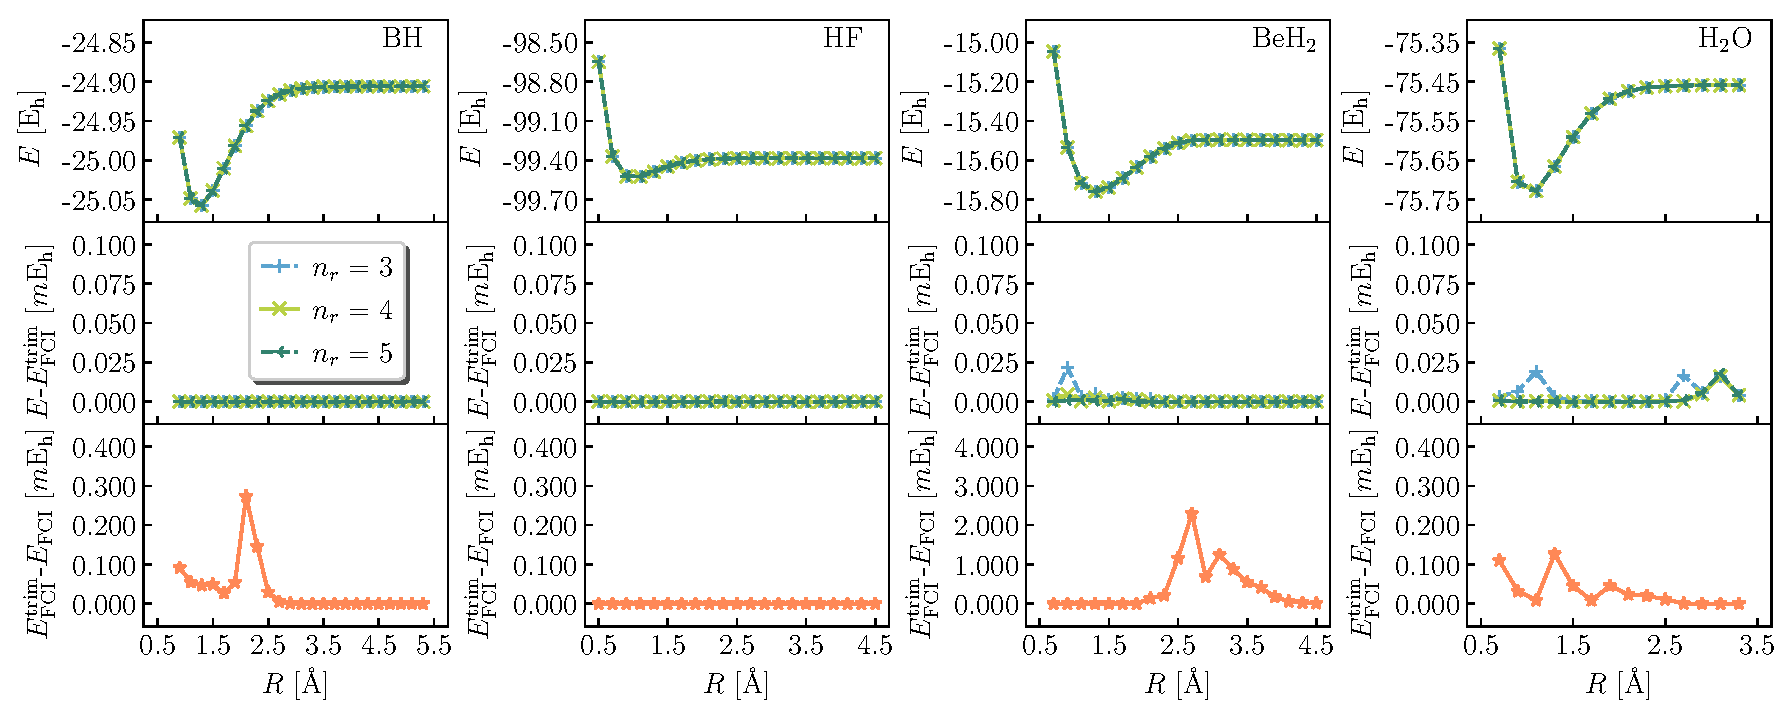
\includegraphics[width=0.9\textwidth]{../figures/first_quantization_trim/first_quantization_trim.eps}
\caption{Total energy, deviation between computed and exact total energy using a first-quantization encoding and a trimming procedure for qubit reduction,
and energy error from the trimming procedure (top to bottom) for the BH, HF, BeH$_2$ and H$_2$O molecules at STO-6G level (left to right) 
using the cascade Ansatz.}
\label{figure:first_trim}
\end{figure} 

\begin{table}[h!]
\begin{tabular}{ccccc|cccc}
\hline\hline
molecule & $n_e=(N_\alpha,N_\beta)$ & $m$ & $n_q$ & $n_p$ & ansatz & $n_{\bgreek{\theta}}$ & $n_g$ & $d$ \\ 
\hline
BH & (4,4) & 5 & 4 & 136 & cascade & $44$ & $(44, 30)$ & $41$ \\ 
\hline
HF & (4,4) & 5 & 3 & 36 & cascade & $33$ & $(33, 20)$ & $31$ \\ 
\hline
BeH$_2$ & (2,2) & 6 & 5 & 528 & cascade & $55$ & $(55, 40)$ & $51$ \\ 
\hline
H$_2$O & (4,4) & 6 & 5 & 528 & cascade & $55$ & $(55, 40)$ & $51$ \\ 
\hline\hline
\end{tabular}
\caption{Computational cost of first-quantization simulations carried out in the present work, using the trimming scheme.
 $n_e$, $m$, $n_q$, and $n_p$ denote numbers of active electrons (spin-up and -down) and orbitals, qubits, and Pauli operators in the Hamiltonian, respectively.
$n_{\bgreek{\theta}}$, $n_g$, and $d$ denote numbers of parameters, gates (single- and two-qubit), and circuit depth. We illustrate the case of $n_r=5$ repetitions.}
\label{table:computational_cost_first_trim}
\end{table}

In Figures \ref{figure:first_pad_vap_cascade} and \ref{figure:first_pad_vap_ry} we we compute ground-state potential energy curves for the BH, HF, BeH$_2$, and H$_2$O molecules 
(left to right), using the "padding" detailed in Appendix \ref{sec:first}, the variation-after-projection optimization, and the cascade and linear-connectivity $\ry$ Ans\"{a}tze respectively.
While the cascade calculations have an accuracy roughly comparable with that of the "trimmed" calculations shown in Figure \ref{figure:first_trim},
the $\ry$ Ansatz reaches milliHartree accuracy featuring multiple cusps.

In both cases, the squared-norm $P$ of the physical component of the wavefunction can reach values as small as $2 \cdot 10^{-1}$ and $1 \cdot 10^{-2}$ for cascade and $\ry$ respectively.
Such a phenomenon indicates that, for both Ans\"{a}tze, lowering the energy is accompanied by leakage of the wavefunction outside the physical subspace.

The computational costs of the first-quantization simulations shown in Figures \ref{figure:first_trim} are listed in Table \ref{table:computational_cost_first_pad}.
The number of qubits is higher than for the trimming scheme, Table \ref{table:computational_cost_first_trim}. Consequently, the Hamiltonian measurement is 
more expensive than in both second quantization and first quantization with trimming.

\begin{figure}[t!]
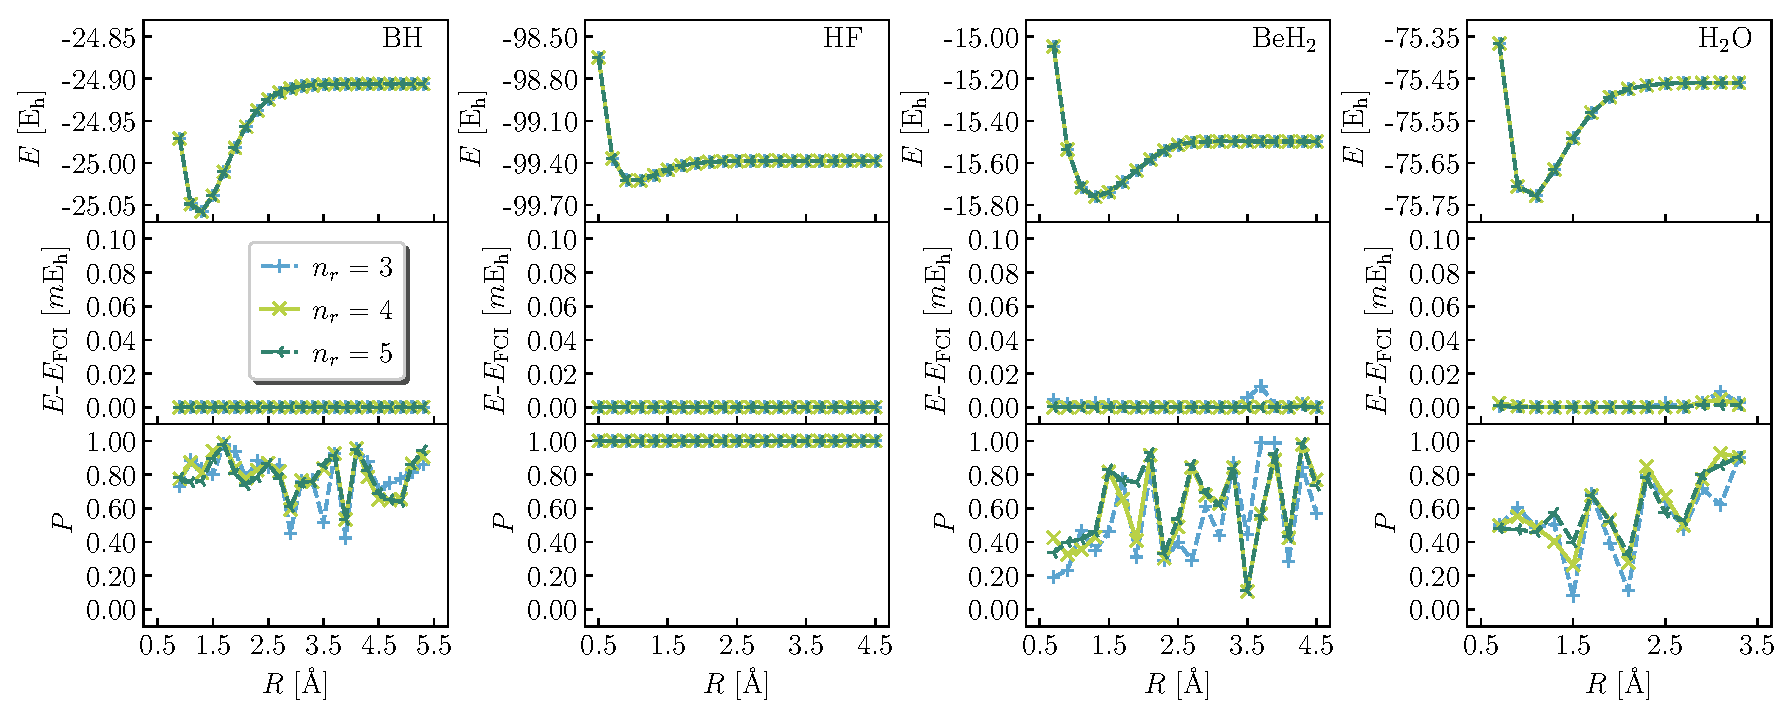
\includegraphics[width=0.9\textwidth]{../figures/first_quantization_pad_vap_cascade/first_quantization_pad_vap_cascade.eps}
\caption{Total energy, deviation between computed and exact energy, and squared-norm of the physical component of the wavefunction
(top to bottom) for the BH, HF, BeH$_2$ and H$_2$O molecules at STO-6G level (left to right) 
using a first-quantization encoding with padding and a cascade Ansatz optimized with the variation-after-projection scheme.}
\label{figure:first_pad_vap_cascade}
\end{figure} 

\begin{figure}[t!]
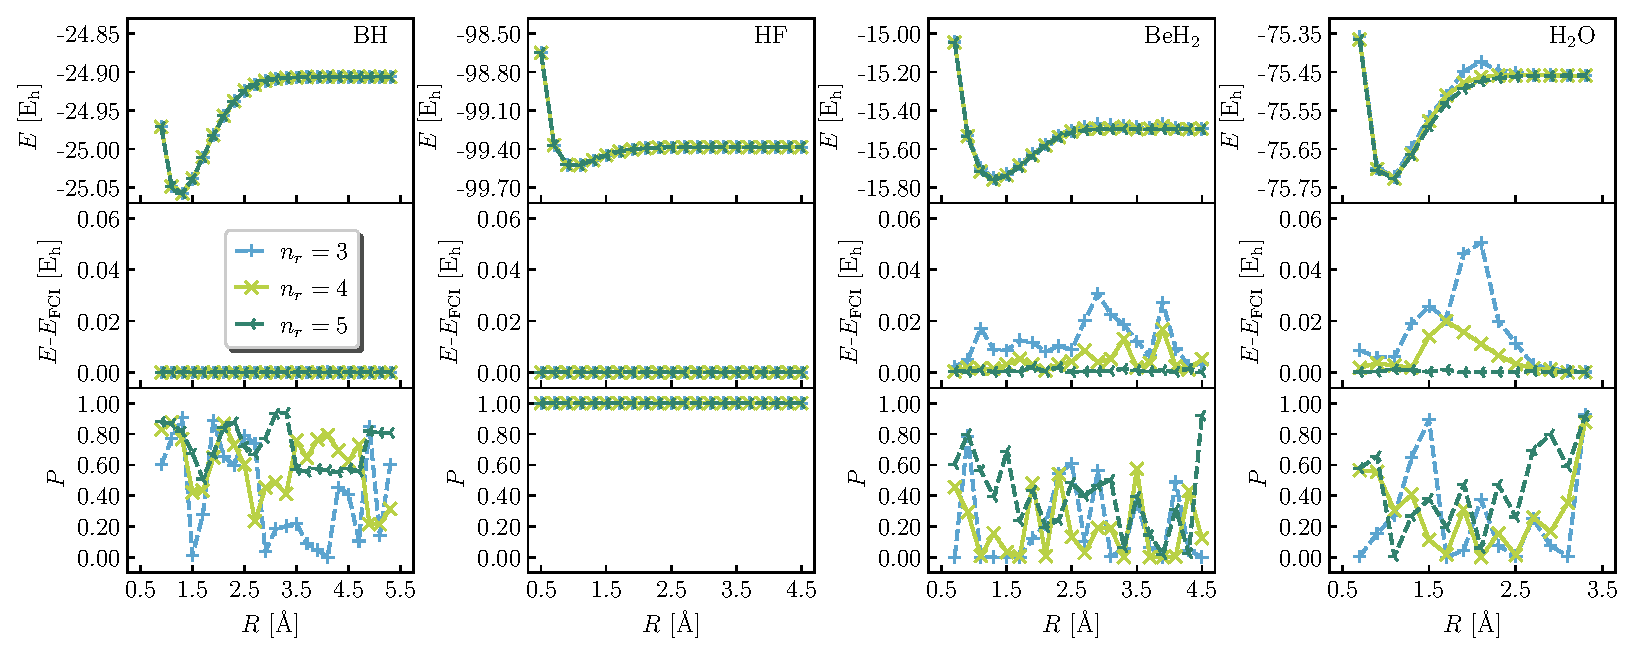
\includegraphics[width=0.9\textwidth]{../figures/first_quantization_pad_vap_ry_linear/first_quantization_pad_vap_ry_linear.eps}
\caption{Total energy, deviation between computed and exact energy, and squared-norm of the physical component of the wavefunction
(top to bottom) for the BH, HF, BeH$_2$ and H$_2$O molecules at STO-6G level (left to right) 
using a first-quantization encoding with padding and an R$_y$ Ansatz with linear connectivity optimized with the variation-after-projection scheme.
}
\label{figure:first_pad_vap_ry}
\end{figure} 

\begin{table}[h!]
\begin{tabular}{ccccc|cccc}
\hline\hline
molecule & $n_e=(N_\alpha,N_\beta)$ & $m$ & $n_q$ & $n_p$ & ansatz & $n_{\bgreek{\theta}}$ & $n_g$ & $d$ \\ 
\hline
BH & (4,4) & 5 & 5 & 480 & $\ry$, linear & $30$ & $(30, 20)$ & $18$ \\ 
  &   &  &   &   & cascade & $55$ & $(55, 40)$ & $51$ \\ 
\hline
HF & (4,4) & 5 & 3 & 36 & $\ry$, linear & $18$ & $(18, 10)$ & $16$ \\ 
  &   &  &   &   & cascade & $33$ & $(33, 20)$ & $31$ \\ 
\hline
BeH$_2$ & (2,2) & 6 & 6 & 2080 & $\ry$, linear & $36$ & $(36, 25)$ & $19$ \\ 
  &   &  &   &   & cascade & $66$ & $(66, 50)$ & $61$ \\ 
\hline
H$_2$O & (4,4) & 6 & 6 & 2080 & $\ry$, linear & $36$ & $(36, 25)$ & $19$ \\ 
  &   &  &   &   & cascade & $66$ & $(66, 50)$ & $61$ \\ 
\hline\hline
\end{tabular}
\caption{Computational cost of first-quantization simulations carried out in the present work, using the padding scheme.
 $n_e$, $m$, $n_q$, and $n_p$ denote numbers of active electrons (spin-up and -down) and orbitals, qubits, and Pauli operators in the Hamiltonian, respectively.
$n_{\bgreek{\theta}}$, $n_g$, and $d$ denote numbers of parameters, gates (single- and two-qubit), and circuit depth. We illustrate the case of $n_r=5$ repetitions.}
\label{table:computational_cost_first_pad}
\end{table}


\section{Conclusions and outlooks}
\label{sec:conclusions}

\todo{write write write write write}

% multireference ansatz (mref vqe by parrish)
% other ansatze (qcc, fabric)
% other algorithms, such as diagonalization (qdf, qse)
% open-shell (radicals)
% non-minimal bases (6-31g)
% more properties (electrostatic)
% other encodings
% hardware (simulators, and error mitigations)

\section*{Acknowledgments}

MM and JER acknowledge the IBM Research Cognitive Computing Cluster service for providing resources that have contributed to the research results reported in this paper.

\appendix

\section{Repository}
\label{sec:github}

\todo{write write write write write}

\section{q-UCCSD}
\label{sec:cc_trotter}

\todo{write write write write write}

\subsection{Closed-shell implementation}

\todo{write write write write write}

\begin{figure}[t!]
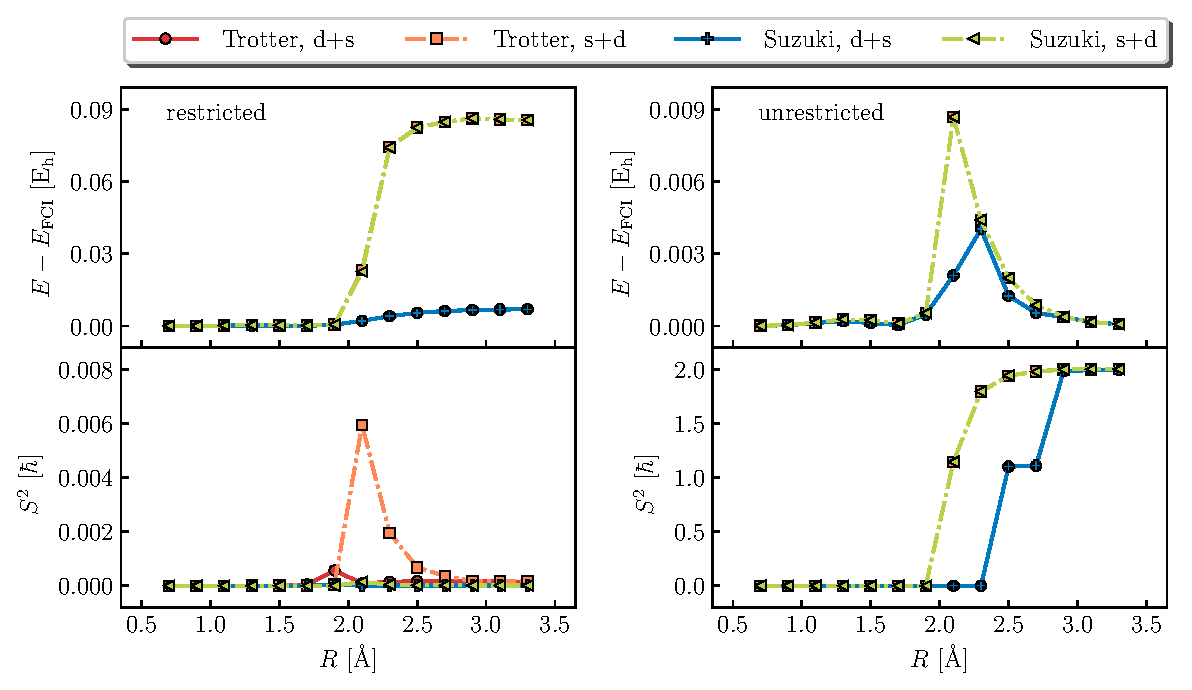
\includegraphics[width=0.7\textwidth]{../figures/qUCCSD_flavors/quccsd_reps_1.eps}
\caption{Deviation between computed and exact energy (top) and total spin (bottom), for the restricted closed-shell (left) and unrestricted (right) qUCCSD Ans\"{a}tze with $n_r=1$ repetitions, for the H$_2$O molecule at STO-6G level, using Trotter and Suzuki approximations (warm, cold colors) and with singles followed by doubles and doubles followed by singles (light, dark colors).}
\label{figure:quccsd_reps_1}
\end{figure} 

\begin{figure}[t!]
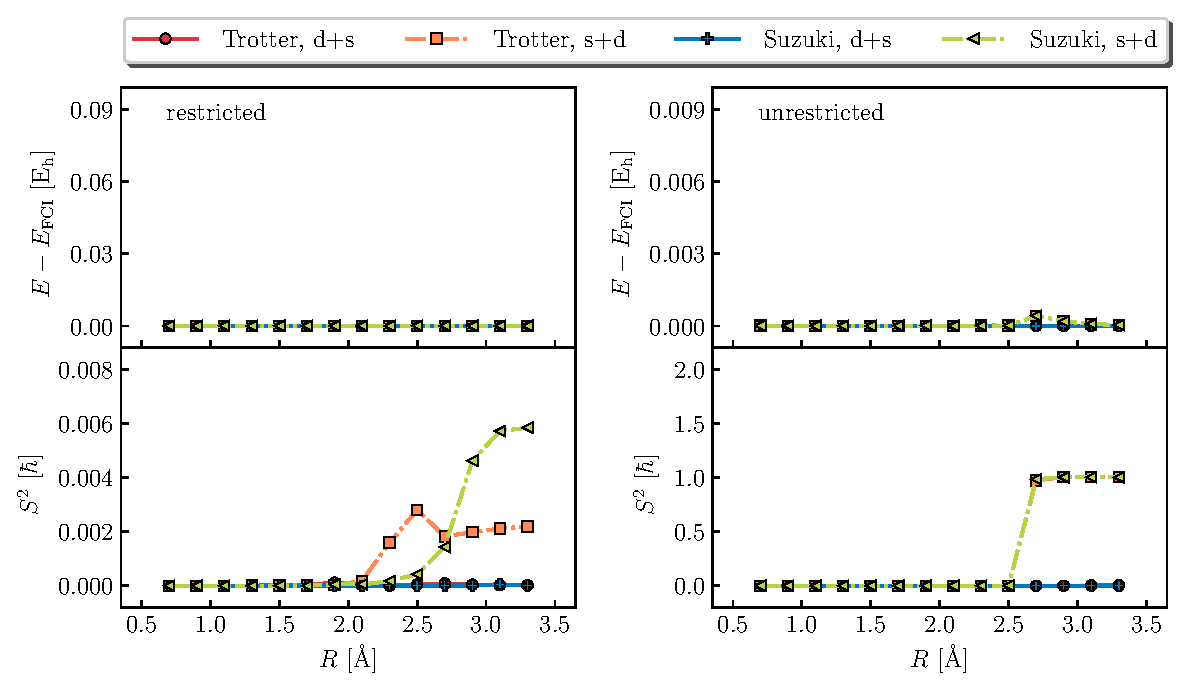
\includegraphics[width=0.7\textwidth]{../figures/qUCCSD_flavors/quccsd_reps_2.eps}
\caption{Deviation between computed and exact energy (top) and total spin (bottom), for the restricted closed-shell (left) and unrestricted (right) qUCCSD Ans\"{a}tze with $n_r=2$ repetitions, for the H$_2$O molecule at STO-6G level, using Trotter and Suzuki approximations (warm, cold colors) and with singles followed by doubles and doubles followed by singles (light, dark colors).}
\label{figure:quccsd_reps_2}
\end{figure} 

\subsection{Primitives}

\todo{write write write write write}

\begin{figure}[t!]
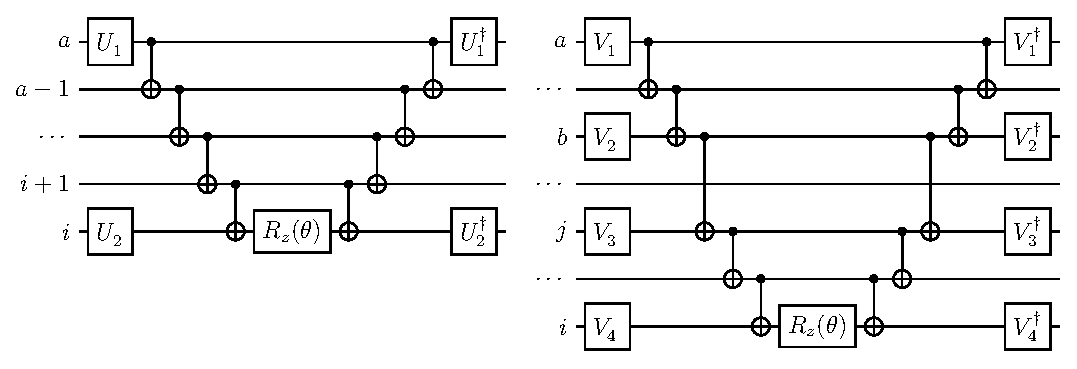
\includegraphics[width=0.7\textwidth]{../figures/circuits/quccsd_primitives.eps}
\caption{
Quantum circuits for the exponentiation of the single (a) and double (b) excitation operators in the q-UCCSD Ansatz  in a Jordan-Wigner representation. 
Indices $a,b,i,j$ label occupied and virtual spin-orbitals, and Clifford unitaries are $(U_1,U_2)=\{(A_Y,A_X)$, $(A_X,A_Y)\}$ for singles,
and
$(V_1,V_2,V_3,V_4) = (A_X,A_X,A_Y,A_X)$, $(A_Y,A_X,A_Y,A_Y)$,
$(A_X,A_Y,A_Y,A_Y)$, $(A_X,A_X,A_X,A_Y)$, $(A_Y,A_X,A_X,A_X)$,
$(A_X,A_Y,A_X,A_X)$, $(A_Y,A_Y,A_Y,A_X)$, $(A_Y,A_Y,A_X,A_Y) \}$
for doubles, with
$A_X = H$ and $A_Y = HS$ and $H$, $S$ denoting the Hadamard and $S$ gates respectively.
}
\label{figure:quccsd_circuit}
\end{figure} 

\section{First quantization encoding}
\label{sec:first}

To carry out simulations in first quantization, we introduce a basis of Slater determinants $\{ {\bf{x}}_i \}_{i=0}^{n_c-1}$ of $n_e=(N_\alpha,N_\beta)$ electrons in $m$ spatial orbitals
(specifically the MOs from a restricted closed-shell HF simulation), i.e. of electronic configurations. 
We then select configurations in the same irrep of the symmetry group to which the HF state belongs, i.e. $A_1$ in the present work.
In the basis of such configurations, we construct the Hamiltonian and total spin matrices
\begin{equation}
H_{ij} = \langle {\bf{x}}_i | \hat{H} | {\bf{x}}_j \rangle
\quad,\quad
S_{ij} = \langle {\bf{x}}_i | \hat{S}^2 | {\bf{x}}_j \rangle
\quad.
\end{equation}
We diagonalize the total spin matrix obtaining a basis of configuration state functions (CSFs), $S_{ij} \phi_{j\mu} = s_\mu \phi_{i\mu}$, out of which we select singlet CSFs 
($\mu$ such that $s_\mu=0$). Finally, we project the Hamiltonian matrix in the singlet subspace, constructing the operator
\begin{equation}
\tilde{H} = \sum_{\mu\nu=0}^{d-1} | \phi_\mu \rangle \langle \phi_\mu | \hat{H} | \phi_\nu \rangle \langle \phi_\nu |
\quad.
\end{equation}
Where $d$ is the number of singlet CSFs in the target irrep. In some cases, $d=2^{n_q}$ for some number of qubits $n_q$, in which case $\tilde{H}$ can be represented as a qubit
operator by expanding it on the Hilbert-Schmidt basis,
\begin{equation}
\tilde{H} = \sum_{\vett{v} \, \vett{w}} \sigma_{\vett{v} \, \vett{w}} \; \frac{ \mbox{Tr}\big[ \sigma_{\vett{v} \, \vett{w}} \tilde{H} \big] }{2^{n_q} } \quad.
\end{equation}
In general, $2^{n_q-1} < d < 2^{n_q}$ for some integer $n_q$, and $\tilde{H}$ can be represented as a qubit operator in at least two ways:
\begin{enumerate}
\item by "trimming" the matrix $\langle \phi_\mu | \hat{H} | \phi_\nu \rangle$ removing a subset of $d-2^{n_q-1}$ CSFs. 
In the present work, we elected to compute the ground-state wavefunction of $\tilde{H}$ and removed the CSFs with smallest coefficients in magnitude.
\item by introducing a set of $2^{n_q}-d$ additional basis functions, called "unphysical" basis function, 
padding the matrix $\langle \phi_\mu | \hat{H} | \phi_\nu \rangle$ to produce a $2^{n_q} \times 2^{n_q}$ matrix, 
and introducing a projector onto the span of "physical" basis functions,
\begin{equation}
J_{\mu\nu} = 
\left(
\begin{array}{c|c}
\tilde{H} & {\bf{0}} \\
\hline
{\bf{0}} & \lambda \mathbbm{1} \\
\end{array} 
\right)
\quad,\quad
\Pi_{\mu\nu} =
\left(
\begin{array}{c|c}
\mathbbm{1} & {\bf{0}} \\
\hline
{\bf{0}} & {\bf{0}} \\
\end{array} 
\right)
\quad .
\end{equation}
\end{enumerate}
In this work, we chose $\lambda = 10^4 \, \mathrm{E_h}$.

\subsection{Variation-after-projection (VAP) and projection-after-variation (PAV) schemes}
\label{sec:pav}

Second-quantization make use of the full Fock space of electrons in $m$ spatial orbitals. 
As observed in Section \ref{sec:results}, this choice can lead to various symmetry breaking phenomena, 
due to qubit wavefunctions having a component outside the target subspace (e.g. $N = N_\alpha + N_\beta$, $S_z = (N_\alpha - N_\beta)/2$,
and $S^2 = S_z (S_z+1) \hbar$).

When first-quantization calculations are carried out within the "padding" scheme, a form of symmetry breaking can occur, 
due to qubit wavefunctions having a component outside the "physical" subspace (the image of the projector $\hat \Pi$).
To avoid such a symmetry breaking, two schemes can be deployed:
\begin{enumerate}
\item Variation-after-projection (VAP). The following cost function is optimized,
\begin{equation}
\label{eq:vap_cost_function}
E_{\mathrm{vap}}(\bgreek{\theta}) = \frac{ \langle \Psi(\bgreek{\theta}) | \hat \Pi \hat{J} \hat \Pi | \Psi(\bgreek{\theta}) \rangle }{ \langle \Psi(\bgreek{\theta}) | \hat\Pi | \Psi(\bgreek{\theta}) \rangle } \quad ,
\end{equation}
i.e. the wavefunction $| \Psi(\bgreek{\theta}) \rangle$ is first projected in the physical subspace, and the energy is then optimized.
\item Projection-after-variation (PAV). The cost function
\begin{equation}
E_{\mathrm{pav}}(\bgreek{\theta}) = \langle \Psi(\bgreek{\theta}) | \hat{J} | \Psi(\bgreek{\theta}) \rangle
\end{equation}
is optimized, and the energy is then computed with Eq. \eqref{eq:vap_cost_function},
i.e. the energy is first optimized, and then re-evaluated over a projected wavefunction.
\end{enumerate}
In Section \ref{sec:results} we focused on the VAP scheme, as it yields more accurate results than PAV.
The PAV scheme is illustrated in Figure \ref{fig:pad_pav} on the BeH$_2$ molecule and the cascade Ansatz. 
Comparison agains the third column of Figure \ref{fig:first_pad_vap_cascade} clearly shows the greater accuracy of the VAP scheme.
It should be noted, however, that both schemes may yield very inaccurate results when the qubit wavefunction lies predominantly
outside the physical subspace, i.e. when $P = \langle \Psi(\bgreek{\theta}) | \hat\Pi | \Psi(\bgreek{\theta}) \rangle \ll 1$.

\begin{figure}[t!]
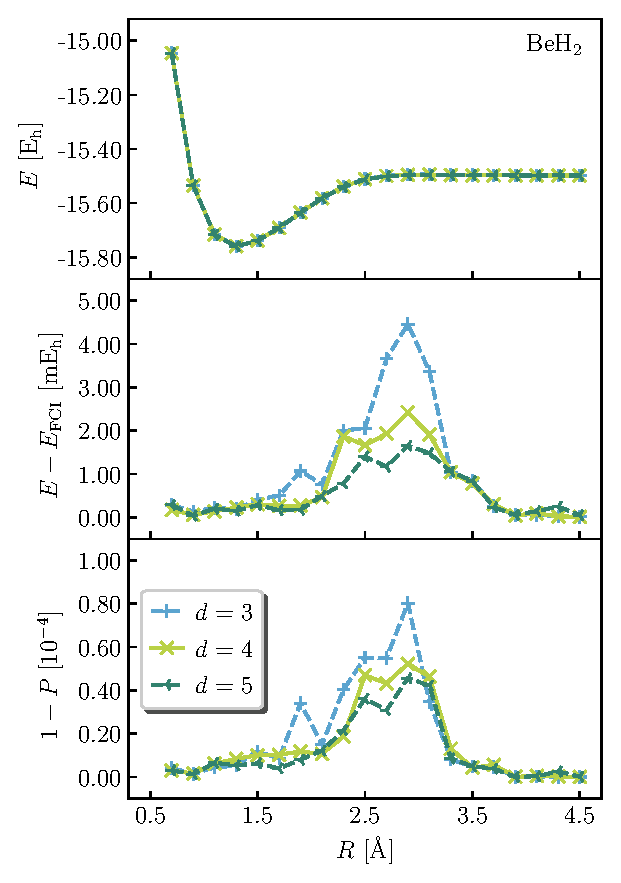
\includegraphics[width=0.4\textwidth]{../figures/first_quantization_pad_pav/first_quantization_pad_pav.eps}
\caption{Total energy, deviation between computed and exact energy, and squared-norm of the unphysical component of the wavefunction
(top to bottom) for the BeH$_2$ molecule at STO-6G level, 
using a first-quantization encoding with padding and a cascade Ansatz optimized with the projection-after-variation scheme.}
\label{figure:pad_pav}
\end{figure} 

\section{Classical preprocessing}
\label{sec:classical}

\todo{write write write write write}

\begin{figure}[t!]
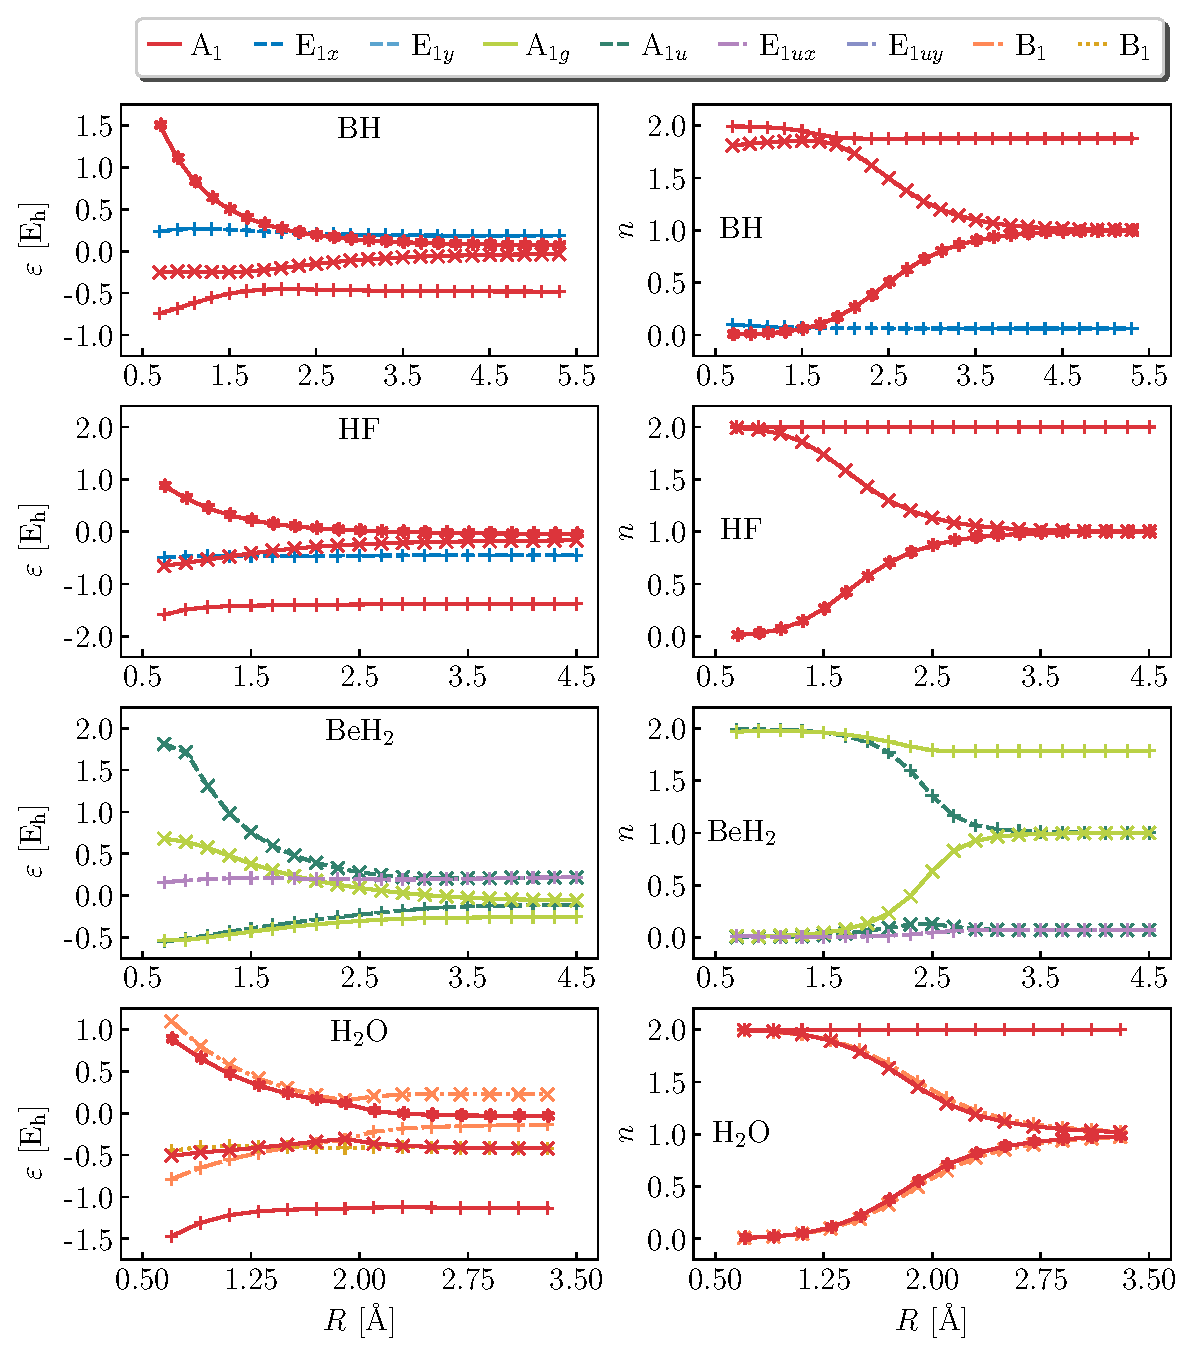
\includegraphics[width=0.6\textwidth]{../figures/scf_fci/scf_fci.eps}
\caption{Eigenvalues of the Fock operator in Hartree units (left, $\varepsilon$) and occupation numbers of the exact ground-state one-body density matrix (right, $n$) 
for BH, HF, BeH$_2$ and H$_2$O (top to bottom). 
Colors denote irreps of the molecular point-group symmetry;
plus, cross, and asterisk markers denote orbitals in ascending order of energy within a specific irrep;
the energy and occupation number of the core 1s orbital are omitted.}
\label{figure:scf}
\end{figure}

\bibliographystyle{apsrev4-2}

\todo{beef up the bibliography}

\bibliography{main}

\end{document}
